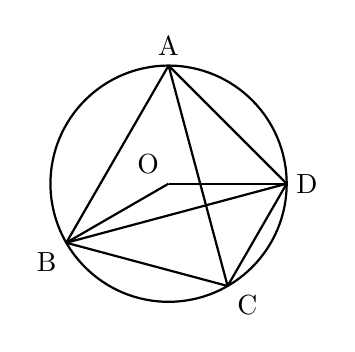
\begin{tikzpicture}[scale=1]
  % Define the center of the circle
  \coordinate (O) at (0,0);

  % Define the radius of the circle
  \def\R{1.5}

  % Draw the circle
  \draw[thick] (O) circle (\R);

  % Define the points on the circle
  % Approximate the angles to match the image
  \coordinate (A) at (90:\R);
  \coordinate (B) at (210:\R);
  \coordinate (C) at (300:\R);
  \coordinate (D) at (0:\R);

  % Draw the line segments connecting the points
  \draw[thick] (A) -- (B);
  \draw[thick] (B) -- (C);
  \draw[thick] (C) -- (D);
  \draw[thick] (D) -- (A);
  
  % Connect A,C line directly
  \draw[thick] (A) -- (C);
  
  % Draw remaining lines (A--O and C--O have been removed)
  \draw[thick] (B) -- (O);
  \draw[thick] (B) -- (D);
  \draw[thick] (D) -- (O);

  % Add labels for the points
  \node[above] at (A) {A};
  \node[below left] at (B) {B};
  \node[below right] at (C) {C};
  \node[right] at (D) {D};
  \node[above left] at (O) {O};

\end{tikzpicture}